\documentclass[1p]{elsarticle_modified}
%\bibliographystyle{elsarticle-num}

%\usepackage[colorlinks]{hyperref}
%\usepackage{abbrmath_seonhwa} %\Abb, \Ascr, \Acal ,\Abf, \Afrak
\usepackage{amsfonts}
\usepackage{amssymb}
\usepackage{amsmath}
\usepackage{amsthm}
\usepackage{scalefnt}
\usepackage{amsbsy}
\usepackage{kotex}
\usepackage{caption}
\usepackage{subfig}
\usepackage{color}
\usepackage{graphicx}
\usepackage{xcolor} %% white, black, red, green, blue, cyan, magenta, yellow
\usepackage{float}
\usepackage{setspace}
\usepackage{hyperref}

\usepackage{tikz}
\usetikzlibrary{arrows}

\usepackage{multirow}
\usepackage{array} % fixed length table
\usepackage{hhline}

%%%%%%%%%%%%%%%%%%%%%
\makeatletter
\renewcommand*\env@matrix[1][\arraystretch]{%
	\edef\arraystretch{#1}%
	\hskip -\arraycolsep
	\let\@ifnextchar\new@ifnextchar
	\array{*\c@MaxMatrixCols c}}
\makeatother %https://tex.stackexchange.com/questions/14071/how-can-i-increase-the-line-spacing-in-a-matrix
%%%%%%%%%%%%%%%

\usepackage[normalem]{ulem}

\newcommand{\msout}[1]{\ifmmode\text{\sout{\ensuremath{#1}}}\else\sout{#1}\fi}
%SOURCE: \msout is \stkout macro in https://tex.stackexchange.com/questions/20609/strikeout-in-math-mode

\newcommand{\cancel}[1]{
	\ifmmode
	{\color{red}\msout{#1}}
	\else
	{\color{red}\sout{#1}}
	\fi
}

\newcommand{\add}[1]{
	{\color{blue}\uwave{#1}}
}

\newcommand{\replace}[2]{
	\ifmmode
	{\color{red}\msout{#1}}{\color{blue}\uwave{#2}}
	\else
	{\color{red}\sout{#1}}{\color{blue}\uwave{#2}}
	\fi
}

\newcommand{\Sol}{\mathcal{S}} %segment
\newcommand{\D}{D} %diagram
\newcommand{\A}{\mathcal{A}} %arc


%%%%%%%%%%%%%%%%%%%%%%%%%%%%%5 test

\def\sl{\operatorname{\textup{SL}}(2,\Cbb)}
\def\psl{\operatorname{\textup{PSL}}(2,\Cbb)}
\def\quan{\mkern 1mu \triangleright \mkern 1mu}

\theoremstyle{definition}
\newtheorem{thm}{Theorem}[section]
\newtheorem{prop}[thm]{Proposition}
\newtheorem{lem}[thm]{Lemma}
\newtheorem{ques}[thm]{Question}
\newtheorem{cor}[thm]{Corollary}
\newtheorem{defn}[thm]{Definition}
\newtheorem{exam}[thm]{Example}
\newtheorem{rmk}[thm]{Remark}
\newtheorem{alg}[thm]{Algorithm}

\newcommand{\I}{\sqrt{-1}}
\begin{document}

%\begin{frontmatter}
%
%\title{Boundary parabolic representations of knots up to 8 crossings}
%
%%% Group authors per affiliation:
%\author{Yunhi Cho} 
%\address{Department of Mathematics, University of Seoul, Seoul, Korea}
%\ead{yhcho@uos.ac.kr}
%
%
%\author{Seonhwa Kim} %\fnref{s_kim}}
%\address{Center for Geometry and Physics, Institute for Basic Science, Pohang, 37673, Korea}
%\ead{ryeona17@ibs.re.kr}
%
%\author{Hyuk Kim}
%\address{Department of Mathematical Sciences, Seoul National University, Seoul 08826, Korea}
%\ead{hyukkim@snu.ac.kr}
%
%\author{Seokbeom Yoon}
%\address{Department of Mathematical Sciences, Seoul National University, Seoul, 08826,  Korea}
%\ead{sbyoon15@snu.ac.kr}
%
%\begin{abstract}
%We find all boundary parabolic representation of knots up to 8 crossings.
%
%\end{abstract}
%\begin{keyword}
%    \MSC[2010] 57M25 
%\end{keyword}
%
%\end{frontmatter}

%\linenumbers
%\tableofcontents
%
\newcommand\colored[1]{\textcolor{white}{\rule[-0.35ex]{0.8em}{1.4ex}}\kern-0.8em\color{red} #1}%
%\newcommand\colored[1]{\textcolor{white}{ #1}\kern-2.17ex	\textcolor{white}{ #1}\kern-1.81ex	\textcolor{white}{ #1}\kern-2.15ex\color{red}#1	}

{\Large $\underline{12n_{0701}~(K12n_{0701})}$}

\setlength{\tabcolsep}{10pt}
\renewcommand{\arraystretch}{1.6}
\vspace{1cm}\begin{tabular}{m{100pt}>{\centering\arraybackslash}m{274pt}}
\multirow{5}{120pt}{
	\centering
	\includegraphics[width=112pt]{../../../GIT/diagram.site/Diagrams/png/2790_12n_0701.png}\\
\ \ \ A knot diagram\footnotemark}&
\allowdisplaybreaks
\textbf{Linearized knot diagam} \\
\cline{2-2}
 &
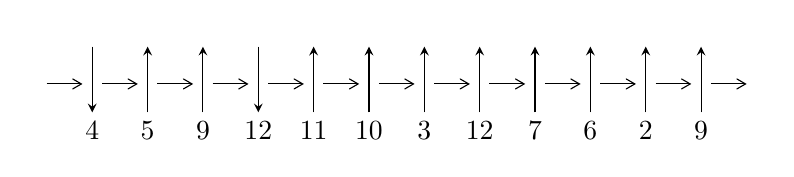
\begin{tikzpicture}[x=20pt, y=17pt]
	% nodes
	\node (C0) at (0, 0) {};
	\node (C1) at (1, 0) {};
	\node (C1U) at (1, +1) {};
	\node (C1D) at (1, -1) {4};

	\node (C2) at (2, 0) {};
	\node (C2U) at (2, +1) {};
	\node (C2D) at (2, -1) {5};

	\node (C3) at (3, 0) {};
	\node (C3U) at (3, +1) {};
	\node (C3D) at (3, -1) {9};

	\node (C4) at (4, 0) {};
	\node (C4U) at (4, +1) {};
	\node (C4D) at (4, -1) {12};

	\node (C5) at (5, 0) {};
	\node (C5U) at (5, +1) {};
	\node (C5D) at (5, -1) {11};

	\node (C6) at (6, 0) {};
	\node (C6U) at (6, +1) {};
	\node (C6D) at (6, -1) {10};

	\node (C7) at (7, 0) {};
	\node (C7U) at (7, +1) {};
	\node (C7D) at (7, -1) {3};

	\node (C8) at (8, 0) {};
	\node (C8U) at (8, +1) {};
	\node (C8D) at (8, -1) {12};

	\node (C9) at (9, 0) {};
	\node (C9U) at (9, +1) {};
	\node (C9D) at (9, -1) {7};

	\node (C10) at (10, 0) {};
	\node (C10U) at (10, +1) {};
	\node (C10D) at (10, -1) {6};

	\node (C11) at (11, 0) {};
	\node (C11U) at (11, +1) {};
	\node (C11D) at (11, -1) {2};

	\node (C12) at (12, 0) {};
	\node (C12U) at (12, +1) {};
	\node (C12D) at (12, -1) {9};
	\node (C13) at (13, 0) {};

	% arrows
	\draw[->,>={angle 60}]
	(C0) edge (C1) (C1) edge (C2) (C2) edge (C3) (C3) edge (C4) (C4) edge (C5) (C5) edge (C6) (C6) edge (C7) (C7) edge (C8) (C8) edge (C9) (C9) edge (C10) (C10) edge (C11) (C11) edge (C12) (C12) edge (C13) ;	\draw[->,>=stealth]
	(C1U) edge (C1D) (C2D) edge (C2U) (C3D) edge (C3U) (C4U) edge (C4D) (C5D) edge (C5U) (C6D) edge (C6U) (C7D) edge (C7U) (C8D) edge (C8U) (C9D) edge (C9U) (C10D) edge (C10U) (C11D) edge (C11U) (C12D) edge (C12U) ;
	\end{tikzpicture} \\
\hhline{~~} \\& 
\textbf{Solving Sequence} \\ \cline{2-2} 
 &
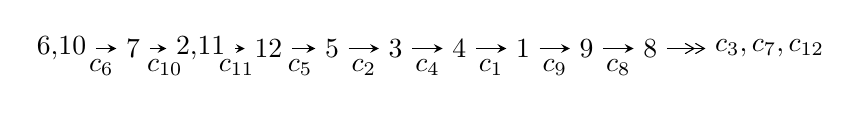
\begin{tikzpicture}[x=23pt, y=7pt]
	% node
	\node (A0) at (-1/8, 0) {6,10};
	\node (A1) at (1, 0) {7};
	\node (A2) at (33/16, 0) {2,11};
	\node (A3) at (25/8, 0) {12};
	\node (A4) at (33/8, 0) {5};
	\node (A5) at (41/8, 0) {3};
	\node (A6) at (49/8, 0) {4};
	\node (A7) at (57/8, 0) {1};
	\node (A8) at (65/8, 0) {9};
	\node (A9) at (73/8, 0) {8};
	\node (C1) at (1/2, -1) {$c_{6}$};
	\node (C2) at (3/2, -1) {$c_{10}$};
	\node (C3) at (21/8, -1) {$c_{11}$};
	\node (C4) at (29/8, -1) {$c_{5}$};
	\node (C5) at (37/8, -1) {$c_{2}$};
	\node (C6) at (45/8, -1) {$c_{4}$};
	\node (C7) at (53/8, -1) {$c_{1}$};
	\node (C8) at (61/8, -1) {$c_{9}$};
	\node (C9) at (69/8, -1) {$c_{8}$};
	\node (A10) at (11, 0) {$c_{3},c_{7},c_{12}$};

	% edge
	\draw[->,>=stealth]	
	(A0) edge (A1) (A1) edge (A2) (A2) edge (A3) (A3) edge (A4) (A4) edge (A5) (A5) edge (A6) (A6) edge (A7) (A7) edge (A8) (A8) edge (A9) ;
	\draw[->>,>={angle 60}]	
	(A9) edge (A10);
\end{tikzpicture} \\ 

\end{tabular} \\

\footnotetext{
The image of knot diagram is generated by the software ``\textbf{Draw programme}" developed by Andrew Bartholomew(\url{http://www.layer8.co.uk/maths/draw/index.htm\#Running-draw}), where we modified some parts for our purpose(\url{https://github.com/CATsTAILs/LinksPainter}).
}\phantom \\ \newline 
\centering \textbf{Ideals for irreducible components\footnotemark of $X_{\text{par}}$} 
 
\begin{align*}
I^u_{1}&=\langle 
u^{22}-5 u^{21}+\cdots+b-3,\;-3 u^{22}+13 u^{21}+\cdots+2 a+22,\;u^{23}-5 u^{22}+\cdots-18 u+2\rangle \\
I^u_{2}&=\langle 
- u^7-5 u^5-7 u^3+u^2+b-2 u+1,\;- u^7- u^6-6 u^5-6 u^4-11 u^3-8 u^2+2 a-5 u-1,\\
\phantom{I^u_{2}}&\phantom{= \langle  }u^8+u^7+6 u^6+4 u^5+11 u^4+4 u^3+7 u^2+u+2\rangle \\
I^u_{3}&=\langle 
- u^8 a+u^8-6 u^6 a+u^7+6 u^6-10 u^4 a+5 u^5- u^3 a+10 u^4-2 u^2 a+7 u^3-3 a u+3 u^2+b+a+2 u,\\
\phantom{I^u_{3}}&\phantom{= \langle  }2 u^9+3 u^8+\cdots-2 a+7,\;u^{10}+u^9+7 u^8+6 u^7+16 u^6+11 u^5+13 u^4+6 u^3+3 u^2+u-1\rangle \\
I^u_{4}&=\langle 
- u^3- u^2+b-2 u-1,\;u^3+a+3 u+2,\;u^4+u^3+3 u^2+3 u+1\rangle \\
\\
\end{align*}
\raggedright * 4 irreducible components of $\dim_{\mathbb{C}}=0$, with total 55 representations.\\
\footnotetext{All coefficients of polynomials are rational numbers. But the coefficients are sometimes approximated in decimal forms when there is not enough margin.}
\newpage
\renewcommand{\arraystretch}{1}
\centering \section*{I. $I^u_{1}= \langle u^{22}-5 u^{21}+\cdots+b-3,\;-3 u^{22}+13 u^{21}+\cdots+2 a+22,\;u^{23}-5 u^{22}+\cdots-18 u+2 \rangle$}
\flushleft \textbf{(i) Arc colorings}\\
\begin{tabular}{m{7pt} m{180pt} m{7pt} m{180pt} }
\flushright $a_{6}=$&$\begin{pmatrix}1\\0\end{pmatrix}$ \\
\flushright $a_{10}=$&$\begin{pmatrix}0\\u\end{pmatrix}$ \\
\flushright $a_{7}=$&$\begin{pmatrix}1\\- u^2\end{pmatrix}$ \\
\flushright $a_{2}=$&$\begin{pmatrix}\frac{3}{2} u^{22}-\frac{13}{2} u^{21}+\cdots+\frac{121}{2} u-11\\- u^{22}+5 u^{21}+\cdots-18 u+3\end{pmatrix}$ \\
\flushright $a_{11}=$&$\begin{pmatrix}u\\u\end{pmatrix}$ \\
\flushright $a_{12}=$&$\begin{pmatrix}-\frac{3}{2} u^{22}+\frac{13}{2} u^{21}+\cdots-\frac{83}{2} u+6\\u^{22}-5 u^{21}+\cdots+24 u-3\end{pmatrix}$ \\
\flushright $a_{5}=$&$\begin{pmatrix}u^2+1\\u^2\end{pmatrix}$ \\
\flushright $a_{3}=$&$\begin{pmatrix}\frac{1}{2} u^{22}-\frac{3}{2} u^{21}+\cdots+\frac{63}{2} u-6\\- u^{22}+5 u^{21}+\cdots-16 u+3\end{pmatrix}$ \\
\flushright $a_{4}=$&$\begin{pmatrix}\frac{1}{2} u^{22}-\frac{3}{2} u^{21}+\cdots+\frac{61}{2} u-6\\- u^{22}+5 u^{21}+\cdots-15 u+3\end{pmatrix}$ \\
\flushright $a_{1}=$&$\begin{pmatrix}\frac{3}{2} u^{22}-\frac{13}{2} u^{21}+\cdots+\frac{81}{2} u-6\\- u^{22}+5 u^{21}+\cdots-23 u+3\end{pmatrix}$ \\
\flushright $a_{9}=$&$\begin{pmatrix}- u\\u^3+u\end{pmatrix}$ \\
\flushright $a_{8}=$&$\begin{pmatrix}-\frac{1}{2} u^{22}+\frac{5}{2} u^{21}+\cdots-\frac{51}{2} u+4\\- u^{15}+3 u^{14}+\cdots+5 u-1\end{pmatrix}$\\&\end{tabular}
\flushleft \textbf{(ii) Obstruction class $= -1$}\\~\\
\flushleft \textbf{(iii) Cusp Shapes $= 6 u^{22}-29 u^{21}+157 u^{20}-513 u^{19}+1582 u^{18}-3829 u^{17}+8406 u^{16}-15713 u^{15}+26319 u^{14}-38607 u^{13}+50328 u^{12}-57710 u^{11}+57948 u^{10}-50468 u^9+37196 u^8-22606 u^7+10398 u^6-2892 u^5-338 u^4+958 u^3-571 u^2+212 u-30$}\\~\\
\newpage\renewcommand{\arraystretch}{1}
\flushleft \textbf{(iv) u-Polynomials at the component}\newline \\
\begin{tabular}{m{50pt}|m{274pt}}
Crossings & \hspace{64pt}u-Polynomials at each crossing \\
\hline $$\begin{aligned}c_{1}\end{aligned}$$&$\begin{aligned}
&u^{23}-14 u^{22}+\cdots+212 u-58
\end{aligned}$\\
\hline $$\begin{aligned}c_{2},c_{11}\end{aligned}$$&$\begin{aligned}
&u^{23}+u^{22}+\cdots+11 u-1
\end{aligned}$\\
\hline $$\begin{aligned}c_{3},c_{8},c_{12}\end{aligned}$$&$\begin{aligned}
&u^{23}+17 u^{21}+\cdots+u-1
\end{aligned}$\\
\hline $$\begin{aligned}c_{4}\end{aligned}$$&$\begin{aligned}
&u^{23}+20 u^{22}+\cdots-7680 u-1024
\end{aligned}$\\
\hline $$\begin{aligned}c_{5},c_{6},c_{9}\\c_{10}\end{aligned}$$&$\begin{aligned}
&u^{23}+5 u^{22}+\cdots-18 u-2
\end{aligned}$\\
\hline $$\begin{aligned}c_{7}\end{aligned}$$&$\begin{aligned}
&u^{23}+u^{22}+\cdots+75 u-76
\end{aligned}$\\
\hline
\end{tabular}\\~\\
\newpage\renewcommand{\arraystretch}{1}
\flushleft \textbf{(v) Riley Polynomials at the component}\newline \\
\begin{tabular}{m{50pt}|m{274pt}}
Crossings & \hspace{64pt}Riley Polynomials at each crossing \\
\hline $$\begin{aligned}c_{1}\end{aligned}$$&$\begin{aligned}
&y^{23}-30 y^{22}+\cdots+95172 y-3364
\end{aligned}$\\
\hline $$\begin{aligned}c_{2},c_{11}\end{aligned}$$&$\begin{aligned}
&y^{23}+15 y^{22}+\cdots+49 y-1
\end{aligned}$\\
\hline $$\begin{aligned}c_{3},c_{8},c_{12}\end{aligned}$$&$\begin{aligned}
&y^{23}+34 y^{22}+\cdots-13 y-1
\end{aligned}$\\
\hline $$\begin{aligned}c_{4}\end{aligned}$$&$\begin{aligned}
&y^{23}+2 y^{22}+\cdots+1835008 y-1048576
\end{aligned}$\\
\hline $$\begin{aligned}c_{5},c_{6},c_{9}\\c_{10}\end{aligned}$$&$\begin{aligned}
&y^{23}+29 y^{22}+\cdots+48 y-4
\end{aligned}$\\
\hline $$\begin{aligned}c_{7}\end{aligned}$$&$\begin{aligned}
&y^{23}+27 y^{22}+\cdots+24929 y-5776
\end{aligned}$\\
\hline
\end{tabular}\\~\\
\newpage\flushleft \textbf{(vi) Complex Volumes and Cusp Shapes}
$$\begin{array}{c|c|c}  
\text{Solutions to }I^u_{1}& \I (\text{vol} + \sqrt{-1}CS) & \text{Cusp shape}\\
 \hline 
\begin{aligned}
u &= \phantom{-}0.642236 + 0.877944 I \\
a &= \phantom{-}0.197001 - 0.148547 I \\
b &= \phantom{-}0.793532 + 0.638924 I\end{aligned}
 & -9.94522 - 0.85971 I & \phantom{-}0.652008 + 0.263340 I \\ \hline\begin{aligned}
u &= \phantom{-}0.642236 - 0.877944 I \\
a &= \phantom{-}0.197001 + 0.148547 I \\
b &= \phantom{-}0.793532 - 0.638924 I\end{aligned}
 & -9.94522 + 0.85971 I & \phantom{-}0.652008 - 0.263340 I \\ \hline\begin{aligned}
u &= \phantom{-}0.525547 + 0.958461 I \\
a &= -0.231366 + 0.083953 I \\
b &= -1.63498 + 0.17452 I\end{aligned}
 & -10.7803 + 10.1203 I & \phantom{-}2.47270 - 6.58788 I \\ \hline\begin{aligned}
u &= \phantom{-}0.525547 - 0.958461 I \\
a &= -0.231366 - 0.083953 I \\
b &= -1.63498 - 0.17452 I\end{aligned}
 & -10.7803 - 10.1203 I & \phantom{-}2.47270 + 6.58788 I \\ \hline\begin{aligned}
u &= \phantom{-}0.808860 + 0.080850 I \\
a &= \phantom{-}0.686984 + 1.110200 I \\
b &= -0.207591 - 0.160006 I\end{aligned}
 & -7.60162 + 5.68429 I & \phantom{-}4.92336 - 4.37173 I \\ \hline\begin{aligned}
u &= \phantom{-}0.808860 - 0.080850 I \\
a &= \phantom{-}0.686984 - 1.110200 I \\
b &= -0.207591 + 0.160006 I\end{aligned}
 & -7.60162 - 5.68429 I & \phantom{-}4.92336 + 4.37173 I \\ \hline\begin{aligned}
u &= \phantom{-}0.024745 + 0.801676 I \\
a &= \phantom{-}0.174801 - 0.754525 I \\
b &= -0.740668 - 0.583637 I\end{aligned}
 & -2.37077 - 1.03630 I & \phantom{-}2.58342 + 3.76841 I \\ \hline\begin{aligned}
u &= \phantom{-}0.024745 - 0.801676 I \\
a &= \phantom{-}0.174801 + 0.754525 I \\
b &= -0.740668 + 0.583637 I\end{aligned}
 & -2.37077 + 1.03630 I & \phantom{-}2.58342 - 3.76841 I \\ \hline\begin{aligned}
u &= \phantom{-}0.180111 + 0.768204 I \\
a &= -0.047351 + 0.934860 I \\
b &= \phantom{-}1.47339 + 0.21993 I\end{aligned}
 & -1.38871 + 3.48902 I & \phantom{-}1.80255 - 2.01978 I \\ \hline\begin{aligned}
u &= \phantom{-}0.180111 - 0.768204 I \\
a &= -0.047351 - 0.934860 I \\
b &= \phantom{-}1.47339 - 0.21993 I\end{aligned}
 & -1.38871 - 3.48902 I & \phantom{-}1.80255 + 2.01978 I\\
 \hline 
 \end{array}$$\newpage$$\begin{array}{c|c|c}  
\text{Solutions to }I^u_{1}& \I (\text{vol} + \sqrt{-1}CS) & \text{Cusp shape}\\
 \hline 
\begin{aligned}
u &= -0.140649 + 1.391640 I \\
a &= \phantom{-}0.471307 - 0.261563 I \\
b &= \phantom{-}0.444719 - 0.537456 I\end{aligned}
 & -3.65805 - 1.94631 I & \phantom{-}9.97208 + 4.88462 I \\ \hline\begin{aligned}
u &= -0.140649 - 1.391640 I \\
a &= \phantom{-}0.471307 + 0.261563 I \\
b &= \phantom{-}0.444719 + 0.537456 I\end{aligned}
 & -3.65805 + 1.94631 I & \phantom{-}9.97208 - 4.88462 I \\ \hline\begin{aligned}
u &= -0.448926\phantom{ +0.000000I} \\
a &= \phantom{-}0.547375\phantom{ +0.000000I} \\
b &= \phantom{-}0.215725\phantom{ +0.000000I}\end{aligned}
 & \phantom{-}0.770537\phantom{ +0.000000I} & \phantom{-}11.8930\phantom{ +0.000000I} \\ \hline\begin{aligned}
u &= \phantom{-}0.01173 + 1.65517 I \\
a &= -1.58298 - 0.41772 I \\
b &= -2.18998 - 0.09600 I\end{aligned}
 & -10.99720 - 0.87329 I & \phantom{-}2.30677 + 2.57929 I \\ \hline\begin{aligned}
u &= \phantom{-}0.01173 - 1.65517 I \\
a &= -1.58298 + 0.41772 I \\
b &= -2.18998 + 0.09600 I\end{aligned}
 & -10.99720 + 0.87329 I & \phantom{-}2.30677 - 2.57929 I \\ \hline\begin{aligned}
u &= \phantom{-}0.04187 + 1.65682 I \\
a &= \phantom{-}2.31152 + 0.13555 I \\
b &= \phantom{-}3.10043 - 0.45940 I\end{aligned}
 & -9.94661 + 4.28907 I & \phantom{-}2.32600 - 1.89884 I \\ \hline\begin{aligned}
u &= \phantom{-}0.04187 - 1.65682 I \\
a &= \phantom{-}2.31152 - 0.13555 I \\
b &= \phantom{-}3.10043 + 0.45940 I\end{aligned}
 & -9.94661 - 4.28907 I & \phantom{-}2.32600 + 1.89884 I \\ \hline\begin{aligned}
u &= \phantom{-}0.286093 + 0.114349 I \\
a &= -0.56165 + 2.23126 I \\
b &= \phantom{-}0.330646 - 0.563761 I\end{aligned}
 & \phantom{-}0.49230 - 1.78185 I & \phantom{-}2.91759 + 6.16768 I \\ \hline\begin{aligned}
u &= \phantom{-}0.286093 - 0.114349 I \\
a &= -0.56165 - 2.23126 I \\
b &= \phantom{-}0.330646 + 0.563761 I\end{aligned}
 & \phantom{-}0.49230 + 1.78185 I & \phantom{-}2.91759 - 6.16768 I \\ \hline\begin{aligned}
u &= \phantom{-}0.14816 + 1.70012 I \\
a &= -2.42737 - 0.12733 I \\
b &= -3.34541 + 0.35416 I\end{aligned}
 & \phantom{-}19.4914 + 12.8043 I & \phantom{-0.000000 } 0. - 5.39440 I\\
 \hline 
 \end{array}$$\newpage$$\begin{array}{c|c|c}  
\text{Solutions to }I^u_{1}& \I (\text{vol} + \sqrt{-1}CS) & \text{Cusp shape}\\
 \hline 
\begin{aligned}
u &= \phantom{-}0.14816 - 1.70012 I \\
a &= -2.42737 + 0.12733 I \\
b &= -3.34541 - 0.35416 I\end{aligned}
 & \phantom{-}19.4914 - 12.8043 I & \phantom{-0.000000 -}0. + 5.39440 I \\ \hline\begin{aligned}
u &= \phantom{-}0.19576 + 1.69910 I \\
a &= \phantom{-}1.23542 + 0.76867 I \\
b &= \phantom{-}1.86806 + 0.82472 I\end{aligned}
 & -18.7857 + 2.4887 I & \phantom{-0.000000 } 0 \\ \hline\begin{aligned}
u &= \phantom{-}0.19576 - 1.69910 I \\
a &= \phantom{-}1.23542 - 0.76867 I \\
b &= \phantom{-}1.86806 - 0.82472 I\end{aligned}
 & -18.7857 - 2.4887 I & \phantom{-0.000000 } 0\\
 \hline 
 \end{array}$$\newpage\newpage\renewcommand{\arraystretch}{1}
\centering \section*{II. $I^u_{2}= \langle - u^7-5 u^5-7 u^3+u^2+b-2 u+1,\;- u^7- u^6+\cdots+2 a-1,\;u^8+u^7+\cdots+u+2 \rangle$}
\flushleft \textbf{(i) Arc colorings}\\
\begin{tabular}{m{7pt} m{180pt} m{7pt} m{180pt} }
\flushright $a_{6}=$&$\begin{pmatrix}1\\0\end{pmatrix}$ \\
\flushright $a_{10}=$&$\begin{pmatrix}0\\u\end{pmatrix}$ \\
\flushright $a_{7}=$&$\begin{pmatrix}1\\- u^2\end{pmatrix}$ \\
\flushright $a_{2}=$&$\begin{pmatrix}\frac{1}{2} u^7+\frac{1}{2} u^6+\cdots+\frac{5}{2} u+\frac{1}{2}\\u^7+5 u^5+7 u^3- u^2+2 u-1\end{pmatrix}$ \\
\flushright $a_{11}=$&$\begin{pmatrix}u\\u\end{pmatrix}$ \\
\flushright $a_{12}=$&$\begin{pmatrix}-\frac{1}{2} u^7-\frac{3}{2} u^6+\cdots-\frac{5}{2} u-\frac{3}{2}\\- u^6- u^5-3 u^4-2 u^3- u^2+1\end{pmatrix}$ \\
\flushright $a_{5}=$&$\begin{pmatrix}u^2+1\\u^2\end{pmatrix}$ \\
\flushright $a_{3}=$&$\begin{pmatrix}\frac{1}{2} u^7+\frac{3}{2} u^6+\cdots+\frac{5}{2} u+\frac{3}{2}\\u^5+2 u^3- u^2-1\end{pmatrix}$ \\
\flushright $a_{4}=$&$\begin{pmatrix}\frac{1}{2} u^7+\frac{3}{2} u^6+\cdots+\frac{3}{2} u+\frac{3}{2}\\u^7+u^6+5 u^5+3 u^4+6 u^3+u^2+u-1\end{pmatrix}$ \\
\flushright $a_{1}=$&$\begin{pmatrix}-\frac{1}{2} u^7-\frac{3}{2} u^6+\cdots-\frac{3}{2} u-\frac{3}{2}\\- u^7-2 u^6-5 u^5-6 u^4-6 u^3-3 u^2- u+1\end{pmatrix}$ \\
\flushright $a_{9}=$&$\begin{pmatrix}- u\\u^3+u\end{pmatrix}$ \\
\flushright $a_{8}=$&$\begin{pmatrix}\frac{1}{2} u^7+\frac{1}{2} u^6+\cdots-\frac{5}{2} u-\frac{5}{2}\\- u^5-2 u^4-4 u^3-5 u^2-3 u-1\end{pmatrix}$\\&\end{tabular}
\flushleft \textbf{(ii) Obstruction class $= 1$}\\~\\
\flushleft \textbf{(iii) Cusp Shapes $= u^7-5 u^6+5 u^5-22 u^4+9 u^3-27 u^2+7 u-6$}\\~\\
\newpage\renewcommand{\arraystretch}{1}
\flushleft \textbf{(iv) u-Polynomials at the component}\newline \\
\begin{tabular}{m{50pt}|m{274pt}}
Crossings & \hspace{64pt}u-Polynomials at each crossing \\
\hline $$\begin{aligned}c_{1}\end{aligned}$$&$\begin{aligned}
&u^8-6 u^7+16 u^6-28 u^5+37 u^4-36 u^3+26 u^2-13 u+4
\end{aligned}$\\
\hline $$\begin{aligned}c_{2},c_{11}\end{aligned}$$&$\begin{aligned}
&u^8+2 u^7+2 u^6-2 u^5-3 u^4-2 u^3+2 u^2+u+1
\end{aligned}$\\
\hline $$\begin{aligned}c_{3},c_{8}\end{aligned}$$&$\begin{aligned}
&u^8- u^7+3 u^6-2 u^5+2 u^3-2 u+1
\end{aligned}$\\
\hline $$\begin{aligned}c_{4}\end{aligned}$$&$\begin{aligned}
&u^8+u^7+2 u^6-2 u^5-3 u^4-2 u^3+2 u^2+2 u+1
\end{aligned}$\\
\hline $$\begin{aligned}c_{5},c_{6}\end{aligned}$$&$\begin{aligned}
&u^8+u^7+6 u^6+4 u^5+11 u^4+4 u^3+7 u^2+u+2
\end{aligned}$\\
\hline $$\begin{aligned}c_{7}\end{aligned}$$&$\begin{aligned}
&u^8+2 u^7+6 u^6+8 u^5+11 u^4+11 u^3+8 u^2+4 u+1
\end{aligned}$\\
\hline $$\begin{aligned}c_{9},c_{10}\end{aligned}$$&$\begin{aligned}
&u^8- u^7+6 u^6-4 u^5+11 u^4-4 u^3+7 u^2- u+2
\end{aligned}$\\
\hline $$\begin{aligned}c_{12}\end{aligned}$$&$\begin{aligned}
&u^8+u^7+3 u^6+2 u^5-2 u^3+2 u+1
\end{aligned}$\\
\hline
\end{tabular}\\~\\
\newpage\renewcommand{\arraystretch}{1}
\flushleft \textbf{(v) Riley Polynomials at the component}\newline \\
\begin{tabular}{m{50pt}|m{274pt}}
Crossings & \hspace{64pt}Riley Polynomials at each crossing \\
\hline $$\begin{aligned}c_{1}\end{aligned}$$&$\begin{aligned}
&y^8-4 y^7-6 y^6+20 y^5+37 y^4+28 y^3+36 y^2+39 y+16
\end{aligned}$\\
\hline $$\begin{aligned}c_{2},c_{11}\end{aligned}$$&$\begin{aligned}
&y^8+6 y^6-4 y^5+7 y^4-8 y^3+2 y^2+3 y+1
\end{aligned}$\\
\hline $$\begin{aligned}c_{3},c_{8},c_{12}\end{aligned}$$&$\begin{aligned}
&y^8+5 y^7+5 y^6+6 y^4-6 y^3+8 y^2-4 y+1
\end{aligned}$\\
\hline $$\begin{aligned}c_{4}\end{aligned}$$&$\begin{aligned}
&y^8+3 y^7+2 y^6-8 y^5+7 y^4-4 y^3+6 y^2+1
\end{aligned}$\\
\hline $$\begin{aligned}c_{5},c_{6},c_{9}\\c_{10}\end{aligned}$$&$\begin{aligned}
&y^8+11 y^7+50 y^6+122 y^5+175 y^4+154 y^3+85 y^2+27 y+4
\end{aligned}$\\
\hline $$\begin{aligned}c_{7}\end{aligned}$$&$\begin{aligned}
&y^8+8 y^7+26 y^6+40 y^5+27 y^4+3 y^3-2 y^2+1
\end{aligned}$\\
\hline
\end{tabular}\\~\\
\newpage\flushleft \textbf{(vi) Complex Volumes and Cusp Shapes}
$$\begin{array}{c|c|c}  
\text{Solutions to }I^u_{2}& \I (\text{vol} + \sqrt{-1}CS) & \text{Cusp shape}\\
 \hline 
\begin{aligned}
u &= -0.369565 + 0.771008 I \\
a &= -0.155753 - 0.334209 I \\
b &= \phantom{-}1.184060 + 0.040896 I\end{aligned}
 & -0.59040 - 4.34638 I & \phantom{-}8.24002 + 7.81362 I \\ \hline\begin{aligned}
u &= -0.369565 - 0.771008 I \\
a &= -0.155753 + 0.334209 I \\
b &= \phantom{-}1.184060 - 0.040896 I\end{aligned}
 & -0.59040 + 4.34638 I & \phantom{-}8.24002 - 7.81362 I \\ \hline\begin{aligned}
u &= \phantom{-}0.201988 + 0.673846 I \\
a &= -1.34000 + 1.00726 I \\
b &= -1.271480 - 0.352014 I\end{aligned}
 & -7.52705 + 0.72220 I & \phantom{-}2.71603 - 0.15399 I \\ \hline\begin{aligned}
u &= \phantom{-}0.201988 - 0.673846 I \\
a &= -1.34000 - 1.00726 I \\
b &= -1.271480 + 0.352014 I\end{aligned}
 & -7.52705 - 0.72220 I & \phantom{-}2.71603 + 0.15399 I \\ \hline\begin{aligned}
u &= -0.23773 + 1.39832 I \\
a &= -0.278315 + 0.491837 I \\
b &= -0.648364 + 0.685778 I\end{aligned}
 & -4.19999 - 1.68332 I & -2.66072 - 1.09034 I \\ \hline\begin{aligned}
u &= -0.23773 - 1.39832 I \\
a &= -0.278315 - 0.491837 I \\
b &= -0.648364 - 0.685778 I\end{aligned}
 & -4.19999 + 1.68332 I & -2.66072 + 1.09034 I \\ \hline\begin{aligned}
u &= -0.09469 + 1.65500 I \\
a &= \phantom{-}2.02407 + 0.03178 I \\
b &= \phantom{-}2.73579 + 0.57245 I\end{aligned}
 & -9.06671 - 6.06893 I & \phantom{-}5.70467 + 5.25665 I \\ \hline\begin{aligned}
u &= -0.09469 - 1.65500 I \\
a &= \phantom{-}2.02407 - 0.03178 I \\
b &= \phantom{-}2.73579 - 0.57245 I\end{aligned}
 & -9.06671 + 6.06893 I & \phantom{-}5.70467 - 5.25665 I\\
 \hline 
 \end{array}$$\newpage\newpage\renewcommand{\arraystretch}{1}
\centering \section*{III. $I^u_{3}= \langle - u^8 a+u^8+\cdots+b+a,\;2 u^9+3 u^8+\cdots-2 a+7,\;u^{10}+u^9+\cdots+u-1 \rangle$}
\flushleft \textbf{(i) Arc colorings}\\
\begin{tabular}{m{7pt} m{180pt} m{7pt} m{180pt} }
\flushright $a_{6}=$&$\begin{pmatrix}1\\0\end{pmatrix}$ \\
\flushright $a_{10}=$&$\begin{pmatrix}0\\u\end{pmatrix}$ \\
\flushright $a_{7}=$&$\begin{pmatrix}1\\- u^2\end{pmatrix}$ \\
\flushright $a_{2}=$&$\begin{pmatrix}a\\u^8 a- u^8+\cdots- a-2 u\end{pmatrix}$ \\
\flushright $a_{11}=$&$\begin{pmatrix}u\\u\end{pmatrix}$ \\
\flushright $a_{12}=$&$\begin{pmatrix}- u^7+u^5 a-4 u^5+3 u^3 a-4 u^3+a u-2 u^2+a-2 u-2\\- u^8 a- u^8+\cdots+a- u\end{pmatrix}$ \\
\flushright $a_{5}=$&$\begin{pmatrix}u^2+1\\u^2\end{pmatrix}$ \\
\flushright $a_{3}=$&$\begin{pmatrix}- u^9 a- u^8 a+\cdots+2 a-1\\- u^8-2 u^7-6 u^6-8 u^5-10 u^4-8 u^3+a u-4 u^2-2 u\end{pmatrix}$ \\
\flushright $a_{4}=$&$\begin{pmatrix}- u^7+u^5 a-4 u^5+3 u^3 a-4 u^3+a u- u^2+a-2 u-1\\- u^8 a- u^8+\cdots+a- u\end{pmatrix}$ \\
\flushright $a_{1}=$&$\begin{pmatrix}- u^9 a- u^8 a+\cdots+3 u+2\\2 u^8 a+2 u^7 a+\cdots+3 a u-2 a\end{pmatrix}$ \\
\flushright $a_{9}=$&$\begin{pmatrix}- u\\u^3+u\end{pmatrix}$ \\
\flushright $a_{8}=$&$\begin{pmatrix}-2 u^9 a-2 u^8 a+\cdots+a+2\\- u^8 a- u^8+\cdots+a- u\end{pmatrix}$\\&\end{tabular}
\flushleft \textbf{(ii) Obstruction class $= -1$}\\~\\
\flushleft \textbf{(iii) Cusp Shapes $= 4 u^8+4 u^7+24 u^6+20 u^5+44 u^4+28 u^3+24 u^2+8 u+2$}\\~\\
\newpage\renewcommand{\arraystretch}{1}
\flushleft \textbf{(iv) u-Polynomials at the component}\newline \\
\begin{tabular}{m{50pt}|m{274pt}}
Crossings & \hspace{64pt}u-Polynomials at each crossing \\
\hline $$\begin{aligned}c_{1}\end{aligned}$$&$\begin{aligned}
&(u^{10}+9 u^9+31 u^8+48 u^7+28 u^6+5 u^5+17 u^4+8 u^3-9 u^2+5 u-1)^2
\end{aligned}$\\
\hline $$\begin{aligned}c_{2},c_{11}\end{aligned}$$&$\begin{aligned}
&u^{20}+9 u^{19}+\cdots+55 u+14
\end{aligned}$\\
\hline $$\begin{aligned}c_{3},c_{8},c_{12}\end{aligned}$$&$\begin{aligned}
&u^{20}- u^{19}+\cdots-109 u+142
\end{aligned}$\\
\hline $$\begin{aligned}c_{4}\end{aligned}$$&$\begin{aligned}
&(u-1)^{20}
\end{aligned}$\\
\hline $$\begin{aligned}c_{5},c_{6},c_{9}\\c_{10}\end{aligned}$$&$\begin{aligned}
&(u^{10}- u^9+7 u^8-6 u^7+16 u^6-11 u^5+13 u^4-6 u^3+3 u^2- u-1)^2
\end{aligned}$\\
\hline $$\begin{aligned}c_{7}\end{aligned}$$&$\begin{aligned}
&u^{20}+u^{19}+\cdots-2452 u+1723
\end{aligned}$\\
\hline
\end{tabular}\\~\\
\newpage\renewcommand{\arraystretch}{1}
\flushleft \textbf{(v) Riley Polynomials at the component}\newline \\
\begin{tabular}{m{50pt}|m{274pt}}
Crossings & \hspace{64pt}Riley Polynomials at each crossing \\
\hline $$\begin{aligned}c_{1}\end{aligned}$$&$\begin{aligned}
&(y^{10}-19 y^9+\cdots-7 y+1)^{2}
\end{aligned}$\\
\hline $$\begin{aligned}c_{2},c_{11}\end{aligned}$$&$\begin{aligned}
&y^{20}- y^{19}+\cdots+2771 y+196
\end{aligned}$\\
\hline $$\begin{aligned}c_{3},c_{8},c_{12}\end{aligned}$$&$\begin{aligned}
&y^{20}+27 y^{19}+\cdots+125859 y+20164
\end{aligned}$\\
\hline $$\begin{aligned}c_{4}\end{aligned}$$&$\begin{aligned}
&(y-1)^{20}
\end{aligned}$\\
\hline $$\begin{aligned}c_{5},c_{6},c_{9}\\c_{10}\end{aligned}$$&$\begin{aligned}
&(y^{10}+13 y^9+\cdots-7 y+1)^{2}
\end{aligned}$\\
\hline $$\begin{aligned}c_{7}\end{aligned}$$&$\begin{aligned}
&y^{20}+23 y^{19}+\cdots+12716706 y+2968729
\end{aligned}$\\
\hline
\end{tabular}\\~\\
\newpage\flushleft \textbf{(vi) Complex Volumes and Cusp Shapes}
$$\begin{array}{c|c|c}  
\text{Solutions to }I^u_{3}& \I (\text{vol} + \sqrt{-1}CS) & \text{Cusp shape}\\
 \hline 
\begin{aligned}
u &= -0.420834 + 0.842935 I \\
a &= \phantom{-}0.198910 - 0.456820 I \\
b &= \phantom{-}1.075440 - 0.460885 I\end{aligned}
 & -1.99815 - 3.55946 I & \phantom{-}1.64226 + 4.06361 I \\ \hline\begin{aligned}
u &= -0.420834 + 0.842935 I \\
a &= \phantom{-}0.291275 - 0.161939 I \\
b &= -1.021720 - 0.224140 I\end{aligned}
 & -1.99815 - 3.55946 I & \phantom{-}1.64226 + 4.06361 I \\ \hline\begin{aligned}
u &= -0.420834 - 0.842935 I \\
a &= \phantom{-}0.198910 + 0.456820 I \\
b &= \phantom{-}1.075440 + 0.460885 I\end{aligned}
 & -1.99815 + 3.55946 I & \phantom{-}1.64226 - 4.06361 I \\ \hline\begin{aligned}
u &= -0.420834 - 0.842935 I \\
a &= \phantom{-}0.291275 + 0.161939 I \\
b &= -1.021720 + 0.224140 I\end{aligned}
 & -1.99815 + 3.55946 I & \phantom{-}1.64226 - 4.06361 I \\ \hline\begin{aligned}
u &= \phantom{-}0.153406 + 0.833677 I \\
a &= \phantom{-}0.02090 - 1.60050 I \\
b &= \phantom{-}0.877616 + 0.641363 I\end{aligned}
 & -8.43900 + 1.60532 I & -3.05654 - 5.03395 I \\ \hline\begin{aligned}
u &= \phantom{-}0.153406 + 0.833677 I \\
a &= -1.42752 + 1.20623 I \\
b &= -2.23360 + 1.38307 I\end{aligned}
 & -8.43900 + 1.60532 I & -3.05654 - 5.03395 I \\ \hline\begin{aligned}
u &= \phantom{-}0.153406 - 0.833677 I \\
a &= \phantom{-}0.02090 + 1.60050 I \\
b &= \phantom{-}0.877616 - 0.641363 I\end{aligned}
 & -8.43900 - 1.60532 I & -3.05654 + 5.03395 I \\ \hline\begin{aligned}
u &= \phantom{-}0.153406 - 0.833677 I \\
a &= -1.42752 - 1.20623 I \\
b &= -2.23360 - 1.38307 I\end{aligned}
 & -8.43900 - 1.60532 I & -3.05654 + 5.03395 I \\ \hline\begin{aligned}
u &= -0.635590\phantom{ +0.000000I} \\
a &= \phantom{-}0.447489 + 0.710048 I \\
b &= \phantom{-}0.228085 - 0.214031 I\end{aligned}
 & \phantom{-}0.553628\phantom{ +0.000000I} & \phantom{-}6.04860\phantom{ +0.000000I} \\ \hline\begin{aligned}
u &= -0.635590\phantom{ +0.000000I} \\
a &= \phantom{-}0.447489 - 0.710048 I \\
b &= \phantom{-}0.228085 + 0.214031 I\end{aligned}
 & \phantom{-}0.553628\phantom{ +0.000000I} & \phantom{-}6.04860\phantom{ +0.000000I}\\
 \hline 
 \end{array}$$\newpage$$\begin{array}{c|c|c}  
\text{Solutions to }I^u_{3}& \I (\text{vol} + \sqrt{-1}CS) & \text{Cusp shape}\\
 \hline 
\begin{aligned}
u &= -0.10787 + 1.66265 I \\
a &= \phantom{-}1.69613 - 0.79881 I \\
b &= \phantom{-}2.25201 - 0.48002 I\end{aligned}
 & -10.67790 - 5.55652 I & -0.20810 + 2.88175 I \\ \hline\begin{aligned}
u &= -0.10787 + 1.66265 I \\
a &= -2.12347 - 0.22802 I \\
b &= -3.08847 - 0.66832 I\end{aligned}
 & -10.67790 - 5.55652 I & -0.20810 + 2.88175 I \\ \hline\begin{aligned}
u &= -0.10787 - 1.66265 I \\
a &= \phantom{-}1.69613 + 0.79881 I \\
b &= \phantom{-}2.25201 + 0.48002 I\end{aligned}
 & -10.67790 + 5.55652 I & -0.20810 - 2.88175 I \\ \hline\begin{aligned}
u &= -0.10787 - 1.66265 I \\
a &= -2.12347 + 0.22802 I \\
b &= -3.08847 + 0.66832 I\end{aligned}
 & -10.67790 + 5.55652 I & -0.20810 - 2.88175 I \\ \hline\begin{aligned}
u &= \phantom{-}0.03425 + 1.67211 I \\
a &= \phantom{-}1.66374 + 1.57382 I \\
b &= \phantom{-}2.49623 + 2.91801 I\end{aligned}
 & -17.3000 + 2.2863 I & -3.60221 - 2.91176 I \\ \hline\begin{aligned}
u &= \phantom{-}0.03425 + 1.67211 I \\
a &= -3.01845 + 1.45580 I \\
b &= -3.46263 + 1.43734 I\end{aligned}
 & -17.3000 + 2.2863 I & -3.60221 - 2.91176 I \\ \hline\begin{aligned}
u &= \phantom{-}0.03425 - 1.67211 I \\
a &= \phantom{-}1.66374 - 1.57382 I \\
b &= \phantom{-}2.49623 - 2.91801 I\end{aligned}
 & -17.3000 - 2.2863 I & -3.60221 + 2.91176 I \\ \hline\begin{aligned}
u &= \phantom{-}0.03425 - 1.67211 I \\
a &= -3.01845 - 1.45580 I \\
b &= -3.46263 - 1.43734 I\end{aligned}
 & -17.3000 - 2.2863 I & -3.60221 + 2.91176 I \\ \hline\begin{aligned}
u &= \phantom{-}0.317683\phantom{ +0.000000I} \\
a &= \phantom{-}2.25101 + 3.10693 I \\
b &= -0.622963 + 0.916801 I\end{aligned}
 & -5.97021\phantom{ +0.000000I} & \phantom{-}8.40060\phantom{ +0.000000I} \\ \hline\begin{aligned}
u &= \phantom{-}0.317683\phantom{ +0.000000I} \\
a &= \phantom{-}2.25101 - 3.10693 I \\
b &= -0.622963 - 0.916801 I\end{aligned}
 & -5.97021\phantom{ +0.000000I} & \phantom{-}8.40060\phantom{ +0.000000I}\\
 \hline 
 \end{array}$$\newpage\newpage\renewcommand{\arraystretch}{1}
\centering \section*{IV. $I^u_{4}= \langle - u^3- u^2+b-2 u-1,\;u^3+a+3 u+2,\;u^4+u^3+3 u^2+3 u+1 \rangle$}
\flushleft \textbf{(i) Arc colorings}\\
\begin{tabular}{m{7pt} m{180pt} m{7pt} m{180pt} }
\flushright $a_{6}=$&$\begin{pmatrix}1\\0\end{pmatrix}$ \\
\flushright $a_{10}=$&$\begin{pmatrix}0\\u\end{pmatrix}$ \\
\flushright $a_{7}=$&$\begin{pmatrix}1\\- u^2\end{pmatrix}$ \\
\flushright $a_{2}=$&$\begin{pmatrix}- u^3-3 u-2\\u^3+u^2+2 u+1\end{pmatrix}$ \\
\flushright $a_{11}=$&$\begin{pmatrix}u\\u\end{pmatrix}$ \\
\flushright $a_{12}=$&$\begin{pmatrix}- u^3- u^2-2 u-1\\- u^2+u\end{pmatrix}$ \\
\flushright $a_{5}=$&$\begin{pmatrix}u^2+1\\u^2\end{pmatrix}$ \\
\flushright $a_{3}=$&$\begin{pmatrix}- u\\u^3+u+1\end{pmatrix}$ \\
\flushright $a_{4}=$&$\begin{pmatrix}u^2- u\\2 u^3+2 u^2+4 u+2\end{pmatrix}$ \\
\flushright $a_{1}=$&$\begin{pmatrix}- u^3-2 u^2-2 u-1\\- u^3-3 u^2-2 u-1\end{pmatrix}$ \\
\flushright $a_{9}=$&$\begin{pmatrix}- u\\u^3+u\end{pmatrix}$ \\
\flushright $a_{8}=$&$\begin{pmatrix}u^2+u+1\\u^2+u\end{pmatrix}$\\&\end{tabular}
\flushleft \textbf{(ii) Obstruction class $= 1$}\\~\\
\flushleft \textbf{(iii) Cusp Shapes $= - u^3+2 u^2-3 u+8$}\\~\\
\newpage\renewcommand{\arraystretch}{1}
\flushleft \textbf{(iv) u-Polynomials at the component}\newline \\
\begin{tabular}{m{50pt}|m{274pt}}
Crossings & \hspace{64pt}u-Polynomials at each crossing \\
\hline $$\begin{aligned}c_{1}\end{aligned}$$&$\begin{aligned}
&u^4-5 u^3+9 u^2-7 u+3
\end{aligned}$\\
\hline $$\begin{aligned}c_{2},c_{11}\end{aligned}$$&$\begin{aligned}
&u^4- u^3+1
\end{aligned}$\\
\hline $$\begin{aligned}c_{3},c_{5},c_{6}\\c_{8}\end{aligned}$$&$\begin{aligned}
&u^4+u^3+3 u^2+3 u+1
\end{aligned}$\\
\hline $$\begin{aligned}c_{4}\end{aligned}$$&$\begin{aligned}
&u^4- u+1
\end{aligned}$\\
\hline $$\begin{aligned}c_{7}\end{aligned}$$&$\begin{aligned}
&u^4-3 u^3+6 u^2-4 u+1
\end{aligned}$\\
\hline $$\begin{aligned}c_{9},c_{10},c_{12}\end{aligned}$$&$\begin{aligned}
&u^4- u^3+3 u^2-3 u+1
\end{aligned}$\\
\hline
\end{tabular}\\~\\
\newpage\renewcommand{\arraystretch}{1}
\flushleft \textbf{(v) Riley Polynomials at the component}\newline \\
\begin{tabular}{m{50pt}|m{274pt}}
Crossings & \hspace{64pt}Riley Polynomials at each crossing \\
\hline $$\begin{aligned}c_{1}\end{aligned}$$&$\begin{aligned}
&y^4-7 y^3+17 y^2+5 y+9
\end{aligned}$\\
\hline $$\begin{aligned}c_{2},c_{11}\end{aligned}$$&$\begin{aligned}
&y^4- y^3+2 y^2+1
\end{aligned}$\\
\hline $$\begin{aligned}c_{3},c_{5},c_{6}\\c_{8},c_{9},c_{10}\\c_{12}\end{aligned}$$&$\begin{aligned}
&y^4+5 y^3+5 y^2-3 y+1
\end{aligned}$\\
\hline $$\begin{aligned}c_{4}\end{aligned}$$&$\begin{aligned}
&y^4+2 y^2- y+1
\end{aligned}$\\
\hline $$\begin{aligned}c_{7}\end{aligned}$$&$\begin{aligned}
&y^4+3 y^3+14 y^2-4 y+1
\end{aligned}$\\
\hline
\end{tabular}\\~\\
\newpage\flushleft \textbf{(vi) Complex Volumes and Cusp Shapes}
$$\begin{array}{c|c|c}  
\text{Solutions to }I^u_{4}& \I (\text{vol} + \sqrt{-1}CS) & \text{Cusp shape}\\
 \hline 
\begin{aligned}
u &= -0.552038 + 0.242275 I \\
a &= -0.272864 - 0.934099 I \\
b &= \phantom{-}0.070951 + 0.424335 I\end{aligned}
 & \phantom{-}1.07586 + 1.18968 I & \phantom{-}10.21923 - 1.46908 I \\ \hline\begin{aligned}
u &= -0.552038 - 0.242275 I \\
a &= -0.272864 + 0.934099 I \\
b &= \phantom{-}0.070951 - 0.424335 I\end{aligned}
 & \phantom{-}1.07586 - 1.18968 I & \phantom{-}10.21923 + 1.46908 I \\ \hline\begin{aligned}
u &= \phantom{-}0.05204 + 1.65794 I \\
a &= -1.72714 - 0.43001 I \\
b &= -2.07095 - 1.05537 I\end{aligned}
 & -15.8803 + 1.6928 I & \phantom{-}2.78077 - 0.08491 I \\ \hline\begin{aligned}
u &= \phantom{-}0.05204 - 1.65794 I \\
a &= -1.72714 + 0.43001 I \\
b &= -2.07095 + 1.05537 I\end{aligned}
 & -15.8803 - 1.6928 I & \phantom{-}2.78077 + 0.08491 I\\
 \hline 
 \end{array}$$\newpage
\newpage\renewcommand{\arraystretch}{1}
\centering \section*{ V. u-Polynomials}
\begin{tabular}{m{50pt}|m{274pt}}
Crossings & \hspace{64pt}u-Polynomials at each crossing \\
\hline $$\begin{aligned}c_{1}\end{aligned}$$&$\begin{aligned}
&(u^4-5 u^3+9 u^2-7 u+3)\\
&\cdot(u^8-6 u^7+16 u^6-28 u^5+37 u^4-36 u^3+26 u^2-13 u+4)\\
&\cdot(u^{10}+9 u^9+31 u^8+48 u^7+28 u^6+5 u^5+17 u^4+8 u^3-9 u^2+5 u-1)^2\\
&\cdot(u^{23}-14 u^{22}+\cdots+212 u-58)
\end{aligned}$\\
\hline $$\begin{aligned}c_{2},c_{11}\end{aligned}$$&$\begin{aligned}
&(u^4- u^3+1)(u^8+2 u^7+2 u^6-2 u^5-3 u^4-2 u^3+2 u^2+u+1)\\
&\cdot(u^{20}+9 u^{19}+\cdots+55 u+14)(u^{23}+u^{22}+\cdots+11 u-1)
\end{aligned}$\\
\hline $$\begin{aligned}c_{3},c_{8}\end{aligned}$$&$\begin{aligned}
&(u^4+u^3+3 u^2+3 u+1)(u^8- u^7+3 u^6-2 u^5+2 u^3-2 u+1)\\
&\cdot(u^{20}- u^{19}+\cdots-109 u+142)(u^{23}+17 u^{21}+\cdots+u-1)
\end{aligned}$\\
\hline $$\begin{aligned}c_{4}\end{aligned}$$&$\begin{aligned}
&((u-1)^{20})(u^4- u+1)(u^8+u^7+\cdots+2 u+1)\\
&\cdot(u^{23}+20 u^{22}+\cdots-7680 u-1024)
\end{aligned}$\\
\hline $$\begin{aligned}c_{5},c_{6}\end{aligned}$$&$\begin{aligned}
&(u^4+u^3+3 u^2+3 u+1)(u^8+u^7+\cdots+u+2)\\
&\cdot(u^{10}- u^9+7 u^8-6 u^7+16 u^6-11 u^5+13 u^4-6 u^3+3 u^2- u-1)^2\\
&\cdot(u^{23}+5 u^{22}+\cdots-18 u-2)
\end{aligned}$\\
\hline $$\begin{aligned}c_{7}\end{aligned}$$&$\begin{aligned}
&(u^4-3 u^3+6 u^2-4 u+1)\\
&\cdot(u^8+2 u^7+6 u^6+8 u^5+11 u^4+11 u^3+8 u^2+4 u+1)\\
&\cdot(u^{20}+u^{19}+\cdots-2452 u+1723)(u^{23}+u^{22}+\cdots+75 u-76)
\end{aligned}$\\
\hline $$\begin{aligned}c_{9},c_{10}\end{aligned}$$&$\begin{aligned}
&(u^4- u^3+3 u^2-3 u+1)(u^8- u^7+\cdots- u+2)\\
&\cdot(u^{10}- u^9+7 u^8-6 u^7+16 u^6-11 u^5+13 u^4-6 u^3+3 u^2- u-1)^2\\
&\cdot(u^{23}+5 u^{22}+\cdots-18 u-2)
\end{aligned}$\\
\hline $$\begin{aligned}c_{12}\end{aligned}$$&$\begin{aligned}
&(u^4- u^3+3 u^2-3 u+1)(u^8+u^7+3 u^6+2 u^5-2 u^3+2 u+1)\\
&\cdot(u^{20}- u^{19}+\cdots-109 u+142)(u^{23}+17 u^{21}+\cdots+u-1)
\end{aligned}$\\
\hline
\end{tabular}\newpage\renewcommand{\arraystretch}{1}
\centering \section*{ VI. Riley Polynomials}
\begin{tabular}{m{50pt}|m{274pt}}
Crossings & \hspace{64pt}Riley Polynomials at each crossing \\
\hline $$\begin{aligned}c_{1}\end{aligned}$$&$\begin{aligned}
&(y^4-7 y^3+17 y^2+5 y+9)\\
&\cdot(y^8-4 y^7-6 y^6+20 y^5+37 y^4+28 y^3+36 y^2+39 y+16)\\
&\cdot((y^{10}-19 y^9+\cdots-7 y+1)^{2})(y^{23}-30 y^{22}+\cdots+95172 y-3364)
\end{aligned}$\\
\hline $$\begin{aligned}c_{2},c_{11}\end{aligned}$$&$\begin{aligned}
&(y^4- y^3+2 y^2+1)(y^8+6 y^6-4 y^5+7 y^4-8 y^3+2 y^2+3 y+1)\\
&\cdot(y^{20}- y^{19}+\cdots+2771 y+196)(y^{23}+15 y^{22}+\cdots+49 y-1)
\end{aligned}$\\
\hline $$\begin{aligned}c_{3},c_{8},c_{12}\end{aligned}$$&$\begin{aligned}
&(y^4+5 y^3+5 y^2-3 y+1)(y^8+5 y^7+\cdots-4 y+1)\\
&\cdot(y^{20}+27 y^{19}+\cdots+125859 y+20164)(y^{23}+34 y^{22}+\cdots-13 y-1)
\end{aligned}$\\
\hline $$\begin{aligned}c_{4}\end{aligned}$$&$\begin{aligned}
&((y-1)^{20})(y^4+2 y^2- y+1)(y^8+3 y^7+\cdots+6 y^2+1)\\
&\cdot(y^{23}+2 y^{22}+\cdots+1835008 y-1048576)
\end{aligned}$\\
\hline $$\begin{aligned}c_{5},c_{6},c_{9}\\c_{10}\end{aligned}$$&$\begin{aligned}
&(y^4+5 y^3+5 y^2-3 y+1)\\
&\cdot(y^8+11 y^7+50 y^6+122 y^5+175 y^4+154 y^3+85 y^2+27 y+4)\\
&\cdot((y^{10}+13 y^9+\cdots-7 y+1)^{2})(y^{23}+29 y^{22}+\cdots+48 y-4)
\end{aligned}$\\
\hline $$\begin{aligned}c_{7}\end{aligned}$$&$\begin{aligned}
&(y^4+3 y^3+14 y^2-4 y+1)\\
&\cdot(y^8+8 y^7+26 y^6+40 y^5+27 y^4+3 y^3-2 y^2+1)\\
&\cdot(y^{20}+23 y^{19}+\cdots+12716706 y+2968729)\\
&\cdot(y^{23}+27 y^{22}+\cdots+24929 y-5776)
\end{aligned}$\\
\hline
\end{tabular}
\vskip 2pc
\end{document}